% chapter 10 - Abhi
\documentclass[../main.tex]{subfiles}

\begin{document}

\section{Parabolic Fixed Points}
\label{sec:10}

We now consider the case when $\lambda$ is a root of unity, $\lambda^r=1$ for $r \in \Q$. In this case, we call $z^*=0$ a \emph{parabolic fixed point}. If $p+1$ is the smallest integer $> 1$ such that $z^{p+1}$ has a non-zero coefficient, we express the analytic map $f$

\begin{equation}
    \label{10:eq:f}
    f(z) = \lambda z + \mu z^{p + 1} + o(z^{p+1})
\end{equation}

In order to characterise the attractive or repulsive nature of the fixed point, we are first interested in finding the \emph{attraction or repulsion directions} to a fixed point.

\subsection{The Case $\lambda = 1$}
If $\lambda = 1$, then the linear part of $f$ is the identity function and so the function behaves like the identity near the fixed point. In this case, $p+1$ is called the \emph{multiplicity} of the fixed point, as it is the multiplicity of the $z=0$ root of $f(z)-z$.

We will first intuitively ponder about the nature of the fixed point in this case, and then formalize our results in Theorem~\ref{10:thm:arvec-ir}.% (The reader is to be warned that everything below until Theorem~\ref{10:thm:arvec-ir} is \emph{non-rigorous}.)
% TODO: don't second person the reader. also, possibly don't attempt to be cute.

% TODO: just replace \alpha with \alpha(\eps).
% TODO: \alpha > 1 / \alpha < 1, fixed point "at" zero
\begin{itemize}
    \item Let $\eps \in \C$ and consider $f(\eps)=\alpha(\eps)\eps$ where $\alpha(\eps)$ is a positive real function of $\eps$ ($\forall \eps, \alpha > 1$ corresponding to repulsion; $\forall \eps, \alpha < 1$ corresponding to attraction). Substituting in Eq.~\ref{10:eq:f} to $p+1$ order in $z$ with $\lambda=1$:
    \begin{equation*}
        {\eps^p} = (\alpha  - 1)/\mu 
    \end{equation*} 
    We can see that there are $p$ \emph{attraction vectors}, which correspond to the argument of $\eps$ when $\alpha < 1$, and $p$ \emph{repulsion vectors}, which correspond to the argument of $\eps$ when $\alpha > 1$. 
    \begin{equation}
        \label{10:eq:v1}
        \begin{array}{*{20}{c}}
            {v_ - ^p =  - 1/(p \mu) } \\
            {v_ + ^p =  + 1/(p \mu) }
        \end{array}    
    \end{equation}
    (The reason for using $1/(p \mu)$ over $1/\mu$ is not important, and will become clear later.)
    Alternatively we may write, where $v_0$ is some repulsion vector, that $v_j$, defined as below, is attractive for odd $j$ and repulsive for even $j$: 
    \begin{equation}
        \label{10:eq:v2}
        v_j = v_0 \exp\left(j/ p \cdot \pi i\right)
    \end{equation}
    \item We may also be interested in asking about the \emph{rate} of convergence of the iteration. Since $\lim_{\eps\tendsto 0}\alpha(\eps) = 1$, which means the convergence is slower than exponential -- in addition, the convergence is slower for larger $p$. We may guess that the sequence $\iter{f}{n}(z)$ converges $\propto v_-/n^{1/p}$.
    \item Taking a cue from the nature of linear dynamical systems, we might imagine the local behaviour of the iterated map to be something like that shown in Fig.~\ref{10:fig:basins}: that the sectors between consecutive repulsion vectors define \emph{attraction basins} for the attraction vector between them -- this would also imply that there are no small cycles near a parabolic fixed point.
\end{itemize}

\begin{figure}
    \label{10:fig:basins}
    \centering
    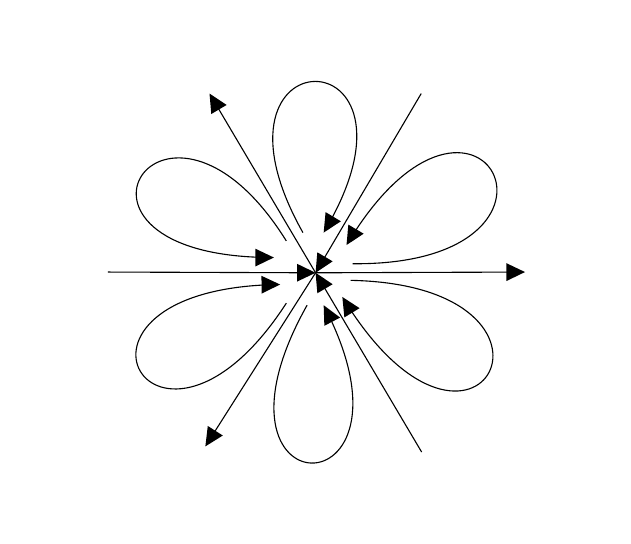
\begin{tikzpicture}[x=0.75pt,y=0.75pt,yscale=-1,xscale=1]
%uncomment if require: \path (0,235); %set diagram left start at 0, and has height of 235

%Straight Lines [id:da7014467597216401] 
\draw    (334,128.64) -- (431.9,128.29) ;
\draw [shift={(434.9,128.28)}, rotate = 539.79] [fill={rgb, 255:red, 0; green, 0; blue, 0 }  ][line width=0.08]  [draw opacity=0] (8.93,-4.29) -- (0,0) -- (8.93,4.29) -- cycle    ;
%Straight Lines [id:da7937079638414151] 
\draw    (334,128.64) -- (284.43,44.86) ;
\draw [shift={(282.9,42.28)}, rotate = 419.39] [fill={rgb, 255:red, 0; green, 0; blue, 0 }  ][line width=0.08]  [draw opacity=0] (8.93,-4.29) -- (0,0) -- (8.93,4.29) -- cycle    ;
%Straight Lines [id:da5652322657720215] 
\draw    (334,128.64) -- (282.51,209.74) ;
\draw [shift={(280.9,212.28)}, rotate = 302.40999999999997] [fill={rgb, 255:red, 0; green, 0; blue, 0 }  ][line width=0.08]  [draw opacity=0] (8.93,-4.29) -- (0,0) -- (8.93,4.29) -- cycle    ;
%Straight Lines [id:da49795176320656886] 
\draw    (384.9,42.28) -- (335.52,126.05) ;
\draw [shift={(334,128.64)}, rotate = 300.51] [fill={rgb, 255:red, 0; green, 0; blue, 0 }  ][line width=0.08]  [draw opacity=0] (8.93,-4.29) -- (0,0) -- (8.93,4.29) -- cycle    ;
%Straight Lines [id:da9443327330326834] 
\draw    (233.9,128.28) -- (331,128.63) ;
\draw [shift={(334,128.64)}, rotate = 180.21] [fill={rgb, 255:red, 0; green, 0; blue, 0 }  ][line width=0.08]  [draw opacity=0] (8.93,-4.29) -- (0,0) -- (8.93,4.29) -- cycle    ;
%Straight Lines [id:da7066291127526734] 
\draw    (385.1,215) -- (335.53,131.22) ;
\draw [shift={(334,128.64)}, rotate = 419.39] [fill={rgb, 255:red, 0; green, 0; blue, 0 }  ][line width=0.08]  [draw opacity=0] (8.93,-4.29) -- (0,0) -- (8.93,4.29) -- cycle    ;
%Curve Lines [id:da8961728852679585] 
\draw    (351.9,124.28) .. controls (472.29,125.27) and (412.51,10.81) .. (349.84,113.71) ;
\draw [shift={(348.9,115.28)}, rotate = 300.82] [fill={rgb, 255:red, 0; green, 0; blue, 0 }  ][line width=0.08]  [draw opacity=0] (8.93,-4.29) -- (0,0) -- (8.93,4.29) -- cycle    ;
%Curve Lines [id:da6878104068351576] 
\draw    (327.9,109.28) .. controls (273.17,12.15) and (394.67,12.65) .. (338.76,107.83) ;
\draw [shift={(337.9,109.28)}, rotate = 300.98] [fill={rgb, 255:red, 0; green, 0; blue, 0 }  ][line width=0.08]  [draw opacity=0] (8.93,-4.29) -- (0,0) -- (8.93,4.29) -- cycle    ;
%Curve Lines [id:da6213553894464128] 
\draw    (319.9,113.28) .. controls (261.19,19.13) and (195.56,120.63) .. (312.13,121.27) ;
\draw [shift={(313.9,121.28)}, rotate = 539.81] [fill={rgb, 255:red, 0; green, 0; blue, 0 }  ][line width=0.08]  [draw opacity=0] (8.93,-4.29) -- (0,0) -- (8.93,4.29) -- cycle    ;
%Curve Lines [id:da5023612601796306] 
\draw    (319.9,143.28) .. controls (257.21,240.17) and (196.51,136.7) .. (315.1,134.3) ;
\draw [shift={(316.9,134.28)}, rotate = 539.3399999999999] [fill={rgb, 255:red, 0; green, 0; blue, 0 }  ][line width=0.08]  [draw opacity=0] (8.93,-4.29) -- (0,0) -- (8.93,4.29) -- cycle    ;
%Curve Lines [id:da5020349766396639] 
\draw    (329.9,144.28) .. controls (273.18,245.15) and (389.72,245.66) .. (338.68,145.79) ;
\draw [shift={(337.9,144.28)}, rotate = 422.4] [fill={rgb, 255:red, 0; green, 0; blue, 0 }  ][line width=0.08]  [draw opacity=0] (8.93,-4.29) -- (0,0) -- (8.93,4.29) -- cycle    ;
%Curve Lines [id:da4534345213536044] 
\draw    (350.9,132.28) .. controls (469.3,134.65) and (411.49,244.55) .. (347.86,141.84) ;
\draw [shift={(346.9,140.28)}, rotate = 418.73] [fill={rgb, 255:red, 0; green, 0; blue, 0 }  ][line width=0.08]  [draw opacity=0] (8.93,-4.29) -- (0,0) -- (8.93,4.29) -- cycle    ;
\end{tikzpicture}

    \caption{Attraction and repulsion vectors, basins where $p = 3$, $\mu\in\R^{> 0}$}
\end{figure}

\begin{thm}
    \label{10:thm:arvec-ir}
    Let $f$ be a holomorphic function with a parabolic fixed point at 0 with multiplier $\lambda = 1$. Let $z_0\in\C$ be such that the sequence $z_n=\iter{f}{n}(z_0)\tendsto 0$ but $\forall n, z_n\ne 0$. Then, for some attraction vector $v_j$ satisfying $v_j^p=-1/(p\mu)$,
    \begin{equation*}
        \lim_{n\tendsto\infty} n^{1/p} z_n = v_j
    \end{equation*}
    i.e. $z_n\sim v_j/n^{1/p}$ asymptotically. $z_n$ is said to tend to 0 \emph{in the direction of $v_j$}.
\end{thm}
\begin{proof}
    The proof relies on a variable substitution $\TrT(z)=-1/(p \mu z^p)$, $\Tr{z}_n=\TrT(z_n)$. Although the substitution is not injective on all of
    % TODO: C \setminus {0}
    $\C\setminus\{0\}$, one may define $2p$ restrictions of the function, $\TrT_j(z):\sector_j\to\C\setminus\R_{(-1)^j}$, where $\sector_j=\{re^{i\theta}v_j : r>0, \abs{\theta} < \pi/p \}$. Then consider the map $\Tr{f}_j(\Tr{z}):=\TrT_j \circ f \circ {\TrT_j}\inv(\Tr{z})$, defined for $\Tr{z}$ outside a large disc on $\C\setminus\R_{(-1)^k}$ -- whose power series it is easy to compute. For simplicity denoting the $p$th root in $\sector_j$ by simply the notation $\sqrt[p]{-}$:
    \begin{align}
        \label{10:eq:fhat}
        f\left(\TrT_j\inv(\Tr{z})\right) &
        = \sqrt[p]{-\frac{1}{p\mu \Tr{z}}}\left(1 - \frac{1}{p\Tr{z}} + o\left(1/\Tr{z} \right)\right)\\
        \TrT \left(f\left(\TrT_j\inv(\Tr{z})\right) \right) &
        = \Tr{z}{\left(1 - \frac{1}{p\Tr{z}} + o\left( {1/\Tr{z}}\right)\right)^{ - p}}\\
        &=\Tr{z}\left(1 + \frac{1}{\Tr{z}} + o\left( {1/\Tr{z}} \right)\right)\\
        &= \Tr{z} + 1 + o(1)
    \end{align}
    \begin{equation}
        \label{10:eq:fhat}
        \Tr{f}_j(\Tr{z}) = \Tr{z} + 1 + o(1)
    \end{equation}
    Then clearly $\Tr{z}_n\sim n$ as $n\tendsto\infty$ (formally: $\Tr{z}_{n+1}-\Tr{z}_n\tendsto 1$, hence the partial sum $(\Tr{z}_n-\Tr{z}_0)/n\tendsto 1$), which implies 
    \begin{equation}
        \label{10:eq:zp}
        z_n^p\sim -1/(p\mu n)
    \end{equation}
    Further, from Eq.~\ref{10:eq:fhat}, $\exists R > 0, \mathrm{Re}(\Tr{z})>R \implies \abs{\Tr{f}_j(\Tr{z})-(\Tr{z}+1)}<1/2$. Then $\Tr{\petal}:=\{\Tr{z}\mid\mathrm{Re}(\Tr{z})>R\}$ is closed under $\Tr{f}_j$, and the \emph{attracting petal} $\petal_j={\TrT_j}\inv\left(\Tr{\petal}\right)$ is closed under $f$. Now since $\exists m, \mathrm{Re}(\Tr{z}_m)>R$, we must have $z_m\in \petal_j$ for some $j$, and by closure of the attracting petal, all further $z_k$ are in this petal. Since by definition $\petal_j\subseteq\sector_j$, this means $z_n$ is eventually in $\sector_j$, and we can take the $n$th root of Eq.~\ref{10:eq:zp}:
    \begin{equation}
        \label{10:eq:z}
        z_n \sim v_j/n^{1/p}
    \end{equation}
\end{proof}
\begin{cor}
    \label{10:cor:arvec-ir-inv}
    Let $z_0$ be such that the sequence $z_n=\inviter{f}{n}(z_0)\tendsto 0$ but $\forall n, z_n\ne 0$. Then, for some repulsion vector $v_j$ of $f$ as defined in Eq.~\ref{10:eq:v2}, $z_n\sim v_j/n^{1/p}$.
\end{cor}

\subsection{The Case $\lambda = \exp(q/r \cdot 2\pi i)$}
Once again, consider $f$ as in Eq.~\ref{10:eq:f}, but with $\lambda$ any primitive $r$th root of unity. Then near its fixed point $z=0$, $f(z)\approx \lambda z$, which for $\lambda\ne 1$ does not have ``true'' attraction and repulsion vectors in the sense that we have been imagining them. 

Instead, we define attraction and repulsion vectors in a way that is more analogous to the notion of limit points, in that we are satisfied with being asymptotic to subsequences.

\begin{dfn}
   Let $f$ be a holomorphic function with parabolic fixed point at 0, and $v$ be a complex number.
    \begin{itemize}
        \item If there exists a sequence $z_n=\iter{f}{n}(z_0)\tendsto 0$ (but $\forall n, z_n\ne 0$) with a subsequence $z_{n_k}$ such that $\arg z_{n_k}\tendsto\arg v$, then $v$ is called an attraction vector for $f$.
        \item If there exists a sequence $z_n=\inviter{f}{n}(z_0)\tendsto 0$ (but $\forall n, z_n\ne 0$) with subsequence $z_{n_k}$ such that $\arg z_{n_k}\tendsto\arg v$, then $v$ is called an repulsion vector for $f$.
    \end{itemize}
\end{dfn}
\begin{thm}
    \label{10:thm:arvec-rot}    
    Let $f$ be a holomorphic function with parabolic fixed point at 0, and multiplier $\lambda=\exp(q/r\cdot 2\pi i)$ where $q/r$ is a fraction in its lowest terms. The attraction vectors of $f$ are the same as the same as those of $\iter{f}{r}$, and their number is a multiple of $r$.
\end{thm}
\begin{proof}
    Any sequence $z_n=\iter{f}{n}(z_0)\tendsto 0$ can be partitioned into subsequences $z_{kr+s}$ for $s=0,\dots r-1$. Each subsequence is an orbit under $\iter{f}{r}$, which is a function of the form discussed in IIIa, thus the attraction vectors of $f$ are precisely those of $\iter{f}{r}$. For each $v$ asymptotic to $z_{kr}$, $\lambda^s v$ is asymptotic to $z_{kr+s}$. Thus any $z_n\tendsto 0$ gives rise to $r$ attraction vectors for $f$. 
\end{proof}
\begin{cor}
    \label{10:thm:rot-mult}
    The multiplicity of the fixed point at 0 of $\iter{f}{r}$ is congruent to 1 mod $r$. 
\end{cor}
Theorem~\ref{10:thm:arvec-rot} is crucial, as it allows us to often reduce problems about parabolic points to the case IIIa. We will be making this without loss of generality assumption about $f$ in sections that follow, and the general case will follow easily through Theorem~\ref{10:thm:arvec-rot}.

\subsection{Petals and Basins}
As we have seen, unlike with attracting and repelling fixed points, parabolic fixed points act in a manner that is simultaneously both attracting and repelling. Thus the notion of an attraction basin in Definition~\ref{intro:dfn:basin} will for the most part be replaced for our purposes by a more specialized Definition~\ref{10:dfn:basin}. Similarly, open neighbourhoods of the origin will often be substituted by the notion of a \emph{petal} per \ref{10:dfn:petal} (although the analogy isn't exact: a superset of a petal is not necessarily a petal).
 
\begin{dfn}
    \label{10:dfn:basin}
    Let $v$ be an attraction vector at fixed point 0. The basin of attraction $\basin_v$ for $v$ is defined as the set of points $z$ such that $\iter{f}{n}(z)\tendsto 0$ in the direction of $v$. The immediate basin of attraction $\basin_v^0$ is defined as the unique connected component of $\basin_v$ that is closed under $f$.
\end{dfn}
\begin{dfn}
    \label{10:dfn:petal}
    Let $f$ be a holomorphic function with parabolic fixed point. Where $f$ is injective on some neighbourhood $\nhd$ of its fixed point, an open set $\petal \subseteq \nhd$ is called an attracting petal for $f$ along attraction vector $v$ if 
    \begin{enumerate} 
        \item $\petal$ is closed under $f$.
        \item $\petal\subseteq\basin_v$
        \item Any orbit $\iter{f}{n}(z_0)$ converging to 0 along $v$ is eventually in $\petal$. 
    \end{enumerate}
\end{dfn}
\begin{lem}
    \label{10:lem:basinopen}
    An attraction basin $\basin_v$ is open.
\end{lem}
\begin{proof}
    We have already seen an example of a petal $\petal$ from the proof of Theorem~\ref{10:thm:arvec-ir} (and one can verify it satisfies the properties). By definition, the orbit of any element $z$ in the attraction basin is eventually in some such $\petal$, i.e. $\iter{f}{n}(z)\in\petal$ for sufficiently large $n$. One may construct a sufficiently small open neighbourhood around $\iter{f}{n}(z)$, and take its preimage under $\iter{f}{n}$ -- by continuity of $\iter{f}{n}$, this preimage must be an open neighbourhood around $z$.  
\end{proof}

The following lemma is analogous to Theorem~\ref{app:lem:julia}.

\begin{lem}
    \label{10:lem:jf}
    For $f$ a holomorphic function with parabolic fixed point, the basins of attraction $\basin_v$ are contained in the Fatou set of $f$, while their boundaries $\partial\basin_v$ are contained in the Julia set.
\end{lem}
\begin{proof}
    By Lemma~\ref{10:lem:basinopen}, $\basin_v$ does not contain its boundary. Thus any $z\in\partial\basin_v$ is not in $\basin_v$. So either: 
    \begin{itemize}
        \item $\iter{f}{n}(z)$ trivially converges to the fixed point, i.e. is eventually 0 (which is in the Julia set due to its proximity to both attracting and repelling orbits). 
        \item $\iter{f}{n}(z)$ does not converge to the fixed point, but is close to points that do, and is therefore in the Julia set.
    \end{itemize}
\end{proof}

We easily arrive at the repulsive version of Definition~\ref{10:dfn:petal} by replacing $f$ with ${f}\inv$.

Somewhat ``better'' petals than the ones used in Theorem~\ref{10:thm:arvec-ir} are formalized in the following theorem: 

\begin{thm}[Parabolic flower theorem]
    \label{10:thm:flower}
    Let $f$ be a holomorphic function as in Eq.~\ref{10:eq:f} with $\lambda = 1$. In any neighbourhood of the fixed point 0, there exist simply connected petals $\petal_{0}\dots\petal_{2p-1}$ (even subscripts repulsive, odd subscripts attractive) such that:
    \begin{itemize}
        \item Their union is a punctured open neighbourhood of 0.
        \item Any two non-adjacent petals are disjoint.
        \item Each $\petal_j$ has a simply-connected region of intersection with $\petal_{j+1}$ and another simply-connected region of intersection with $\petal_{j-1}$.
    \end{itemize}
\end{thm}
(When $p + 1 = 2$, the right- and left- neighbours are the same, but there are still two simply-connected regions of intersection.)
\begin{proof}
    Recall the substitution $\TrT$, and the defined quantity $R$, in the proof of Theorem~\ref{10:thm:arvec-ir}. Then define $\Tr{\petal}^-:=\{x+iy\mid x+\abs{y}>2R\}$ and $\Tr{\petal}^+:=-\Tr{\petal}^-$. Then define:
    \begin{equation*}
        \petal_j=
        \begin{cases} 
            {\TrT_j}\inv(\Tr{\petal}^+) & j\,\,\mathrm{even} \\
            {\TrT_j}\inv(\Tr{\petal}^-) & j\,\,\mathrm{odd}
        \end{cases}
    \end{equation*}
    One can check that the even and odd petals are indeed repulsive and attractive respectively. Each of the required statements can be verified rather easily:
    \begin{itemize}
        \item Since $\Tr{\petal}^+\cup\Tr{\petal}^-$ contains all complex numbers with a radius over $2R$, each petal $\petal_j$ contains a sector centered at the fixed point, of angle spanning $\sector_j$ and radius $(2Rp\mu)^{-1/p}$, Thus their union covers all such sectors, i.e. an open disc. 
        \item Non-adjacent $\sector_j$ are disjoint, and each $\petal_j\subseteq\sector_j$. 
        \item $\Tr{\petal}^+\cap\Tr{\petal}^-=\Tr{\kettle}^\vee\cap\Tr{\kettle}^\wedge$ where the right-hand-side is a disjoint union, $\kettle^\vee = \{x+iy\mid y - \abs{x} > 2R\}$ and $\kettle^\wedge=-\kettle^\vee$. These regions correspond to the intersections of $\petal_j$ with each of its neighbouring petals, i.e. $\TrT(\petal_j\cap\petal_{j+1})$ is either $\kettle^\vee$ or $\kettle^\wedge$ depending on the parity of $j$.
    \end{itemize}
\end{proof}

\begin{figure}
    \label{10:fig:petals}
    \centering
    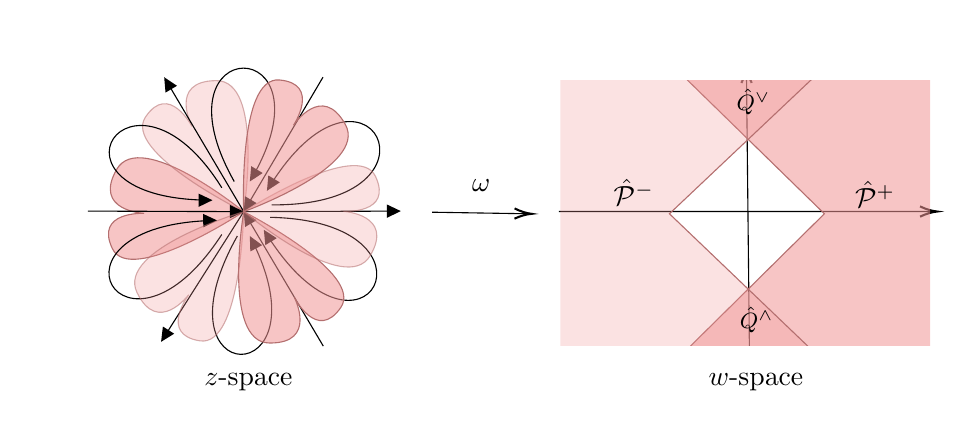
\begin{tikzpicture}[x=0.75pt,y=0.75pt,yscale=-0.75,xscale=0.75]
%uncomment if require: \path (0,286); %set diagram left start at 0, and has height of 286

%Shape: Regular Polygon [id:dp057437658287642135] 
\draw  [color={rgb, 255:red, 180; green, 111; blue, 111 }  ,draw opacity=1 ][fill={rgb, 255:red, 240; green, 149; blue, 149 }  ,fill opacity=0.55 ] (114.98,118.73) .. controls (114.98,118.73) and (82,117.27) .. (97.38,90.48) .. controls (112.76,63.7) and (179,117.64) .. (179,117.64) .. controls (179,117.64) and (106.31,165.61) .. (94.65,141.45) .. controls (83,117.28) and (114.98,118.73) .. (114.98,118.73) -- cycle ;
%Shape: Regular Polygon [id:dp12933226822826427] 
\draw  [color={rgb, 255:red, 180; green, 111; blue, 111 }  ,draw opacity=0.55 ][fill={rgb, 255:red, 240; green, 149; blue, 149 }  ,fill opacity=0.27 ] (145.77,62.9) .. controls (145.77,62.9) and (130.41,33.68) .. (161.29,33.46) .. controls (192.18,33.23) and (179,117.64) .. (179,117.64) .. controls (179,117.64) and (100.92,79.06) .. (115.91,56.81) .. controls (130.9,34.55) and (145.77,62.9) .. (145.77,62.9) -- cycle ;
%Straight Lines [id:da7014467597216401] 
\draw    (179,117.64) -- (276.9,117.29) ;
\draw [shift={(279.9,117.28)}, rotate = 539.79] [fill={rgb, 255:red, 0; green, 0; blue, 0 }  ][line width=0.08]  [draw opacity=0] (8.93,-4.29) -- (0,0) -- (8.93,4.29) -- cycle    ;
%Straight Lines [id:da7937079638414151] 
\draw    (179,117.64) -- (129.43,33.86) ;
\draw [shift={(127.9,31.28)}, rotate = 419.39] [fill={rgb, 255:red, 0; green, 0; blue, 0 }  ][line width=0.08]  [draw opacity=0] (8.93,-4.29) -- (0,0) -- (8.93,4.29) -- cycle    ;
%Straight Lines [id:da5652322657720215] 
\draw    (179,117.64) -- (127.51,198.74) ;
\draw [shift={(125.9,201.28)}, rotate = 302.40999999999997] [fill={rgb, 255:red, 0; green, 0; blue, 0 }  ][line width=0.08]  [draw opacity=0] (8.93,-4.29) -- (0,0) -- (8.93,4.29) -- cycle    ;
%Straight Lines [id:da49795176320656886] 
\draw    (229.9,31.28) -- (180.52,115.05) ;
\draw [shift={(179,117.64)}, rotate = 300.51] [fill={rgb, 255:red, 0; green, 0; blue, 0 }  ][line width=0.08]  [draw opacity=0] (8.93,-4.29) -- (0,0) -- (8.93,4.29) -- cycle    ;
%Straight Lines [id:da9443327330326834] 
\draw    (78.9,117.28) -- (176,117.63) ;
\draw [shift={(179,117.64)}, rotate = 180.21] [fill={rgb, 255:red, 0; green, 0; blue, 0 }  ][line width=0.08]  [draw opacity=0] (8.93,-4.29) -- (0,0) -- (8.93,4.29) -- cycle    ;
%Straight Lines [id:da7066291127526734] 
\draw    (230.1,204) -- (180.53,120.22) ;
\draw [shift={(179,117.64)}, rotate = 419.39] [fill={rgb, 255:red, 0; green, 0; blue, 0 }  ][line width=0.08]  [draw opacity=0] (8.93,-4.29) -- (0,0) -- (8.93,4.29) -- cycle    ;
%Curve Lines [id:da8961728852679585] 
\draw    (196.9,113.28) .. controls (317.29,114.27) and (257.51,-0.19) .. (194.84,102.71) ;
\draw [shift={(193.9,104.28)}, rotate = 300.82] [fill={rgb, 255:red, 0; green, 0; blue, 0 }  ][line width=0.08]  [draw opacity=0] (8.93,-4.29) -- (0,0) -- (8.93,4.29) -- cycle    ;
%Curve Lines [id:da6878104068351576] 
\draw    (172.9,98.28) .. controls (118.17,1.15) and (239.67,1.65) .. (183.76,96.83) ;
\draw [shift={(182.9,98.28)}, rotate = 300.98] [fill={rgb, 255:red, 0; green, 0; blue, 0 }  ][line width=0.08]  [draw opacity=0] (8.93,-4.29) -- (0,0) -- (8.93,4.29) -- cycle    ;
%Curve Lines [id:da6213553894464128] 
\draw    (164.9,102.28) .. controls (106.19,8.13) and (40.56,109.63) .. (157.13,110.27) ;
\draw [shift={(158.9,110.28)}, rotate = 539.81] [fill={rgb, 255:red, 0; green, 0; blue, 0 }  ][line width=0.08]  [draw opacity=0] (8.93,-4.29) -- (0,0) -- (8.93,4.29) -- cycle    ;
%Curve Lines [id:da5023612601796306] 
\draw    (164.9,132.28) .. controls (102.21,229.17) and (41.51,125.7) .. (160.1,123.3) ;
\draw [shift={(161.9,123.28)}, rotate = 539.3399999999999] [fill={rgb, 255:red, 0; green, 0; blue, 0 }  ][line width=0.08]  [draw opacity=0] (8.93,-4.29) -- (0,0) -- (8.93,4.29) -- cycle    ;
%Curve Lines [id:da5020349766396639] 
\draw    (174.9,133.28) .. controls (118.18,234.15) and (234.72,234.66) .. (183.68,134.79) ;
\draw [shift={(182.9,133.28)}, rotate = 422.4] [fill={rgb, 255:red, 0; green, 0; blue, 0 }  ][line width=0.08]  [draw opacity=0] (8.93,-4.29) -- (0,0) -- (8.93,4.29) -- cycle    ;
%Curve Lines [id:da4534345213536044] 
\draw    (195.9,121.28) .. controls (314.3,123.65) and (256.49,233.55) .. (192.86,130.84) ;
\draw [shift={(191.9,129.28)}, rotate = 418.73] [fill={rgb, 255:red, 0; green, 0; blue, 0 }  ][line width=0.08]  [draw opacity=0] (8.93,-4.29) -- (0,0) -- (8.93,4.29) -- cycle    ;
%Shape: Regular Polygon [id:dp7606065427728967] 
\draw  [color={rgb, 255:red, 180; green, 111; blue, 111 }  ,draw opacity=0.55 ][fill={rgb, 255:red, 240; green, 149; blue, 149 }  ,fill opacity=0.27 ] (143.66,171.03) .. controls (143.66,171.03) and (123.78,197.39) .. (110.41,169.55) .. controls (97.03,141.71) and (179,117.64) .. (179,117.64) .. controls (179,117.64) and (177.4,204.71) .. (150.88,200.64) .. controls (124.36,196.57) and (143.66,171.03) .. (143.66,171.03) -- cycle ;
%Shape: Regular Polygon [id:dp10499407073436307] 
\draw  [color={rgb, 255:red, 180; green, 111; blue, 111 }  ,draw opacity=1 ][fill={rgb, 255:red, 240; green, 149; blue, 149 }  ,fill opacity=0.55 ] (211.54,172.79) .. controls (211.54,172.79) and (226.53,202.2) .. (195.65,202.03) .. controls (164.76,201.87) and (179,117.64) .. (179,117.64) .. controls (179,117.64) and (256.59,157.19) .. (241.32,179.26) .. controls (226.05,201.32) and (211.54,172.79) .. (211.54,172.79) -- cycle ;
%Shape: Regular Polygon [id:dp8804803151402205] 
\draw  [color={rgb, 255:red, 180; green, 111; blue, 111 }  ,draw opacity=0.55 ][fill={rgb, 255:red, 240; green, 149; blue, 149 }  ,fill opacity=0.27 ] (243.03,117.46) .. controls (243.03,117.46) and (275.99,119.4) .. (260.23,145.96) .. controls (244.47,172.52) and (179,117.64) .. (179,117.64) .. controls (179,117.64) and (252.36,70.71) .. (263.68,95.04) .. controls (274.99,119.37) and (243.03,117.46) .. (243.03,117.46) -- cycle ;
%Shape: Regular Polygon [id:dp31635047471359634] 
\draw  [color={rgb, 255:red, 180; green, 111; blue, 111 }  ,draw opacity=1 ][fill={rgb, 255:red, 240; green, 149; blue, 149 }  ,fill opacity=0.55 ] (210.97,62.16) .. controls (210.97,62.16) and (229.18,34.62) .. (244.25,61.58) .. controls (259.32,88.54) and (179,117.64) .. (179,117.64) .. controls (179,117.64) and (175.2,30.63) .. (201.93,33.05) .. controls (228.65,35.47) and (210.97,62.16) .. (210.97,62.16) -- cycle ;
%Straight Lines [id:da8740701060140308] 
\draw    (503.9,211.04) -- (501.92,26.04) ;
\draw [shift={(501.9,24.04)}, rotate = 449.39] [color={rgb, 255:red, 0; green, 0; blue, 0 }  ][line width=0.75]    (10.93,-3.29) .. controls (6.95,-1.4) and (3.31,-0.3) .. (0,0) .. controls (3.31,0.3) and (6.95,1.4) .. (10.93,3.29)   ;
%Straight Lines [id:da9217871639595665] 
\draw    (381.4,117.52) -- (622.4,117.56) ;
\draw [shift={(624.4,117.56)}, rotate = 180.01] [color={rgb, 255:red, 0; green, 0; blue, 0 }  ][line width=0.75]    (10.93,-3.29) .. controls (6.95,-1.4) and (3.31,-0.3) .. (0,0) .. controls (3.31,0.3) and (6.95,1.4) .. (10.93,3.29)   ;
%Straight Lines [id:da17434601685188045] 
\draw [color={rgb, 255:red, 180; green, 111; blue, 111 }  ,draw opacity=1 ][fill={rgb, 255:red, 240; green, 149; blue, 149 }  ,fill opacity=0.55 ]   (619.9,209.04) -- (461.9,208.04) -- (552,119) -- (461.9,31.04) -- (619.9,29.04) ;
%Shape: Rectangle [id:dp9982084508684994] 
\draw  [draw opacity=0][fill={rgb, 255:red, 255; green, 255; blue, 255 }  ,fill opacity=1 ] (445,6) -- (625.9,6) -- (625.9,33.04) -- (445,33.04) -- cycle ;
%Shape: Rectangle [id:dp261442729168085] 
\draw  [draw opacity=0][fill={rgb, 255:red, 255; green, 255; blue, 255 }  ,fill opacity=1 ] (452,204) -- (632.9,204) -- (632.9,231.04) -- (452,231.04) -- cycle ;
%Straight Lines [id:da4321981089701783] 
\draw [color={rgb, 255:red, 180; green, 111; blue, 111 }  ,draw opacity=1 ][fill={rgb, 255:red, 240; green, 149; blue, 149 }  ,fill opacity=0.27 ]   (382.33,209.04) -- (545.54,208.04) -- (452.47,119) -- (545.54,31.04) -- (446.39,29.83) -- (382.33,29.04) ;
%Shape: Rectangle [id:dp1675953452553458] 
\draw  [draw opacity=0][fill={rgb, 255:red, 255; green, 255; blue, 255 }  ,fill opacity=1 ] (563,6) -- (376.13,6) -- (376.13,33.04) -- (563,33.04) -- cycle ;
%Shape: Rectangle [id:dp26924443276601817] 
\draw  [draw opacity=0][fill={rgb, 255:red, 255; green, 255; blue, 255 }  ,fill opacity=1 ] (555.77,204) -- (368.9,204) -- (368.9,231.04) -- (555.77,231.04) -- cycle ;
%Straight Lines [id:da5027547130138361] 
\draw    (300,118) -- (361.9,119.01) ;
\draw [shift={(363.9,119.04)}, rotate = 180.93] [color={rgb, 255:red, 0; green, 0; blue, 0 }  ][line width=0.75]    (10.93,-3.29) .. controls (6.95,-1.4) and (3.31,-0.3) .. (0,0) .. controls (3.31,0.3) and (6.95,1.4) .. (10.93,3.29)   ;

% Text Node
\draw (152,220) node [anchor=north west][inner sep=0.75pt]   [align=left] {$\displaystyle z$-space};
% Text Node
\draw (476,220) node [anchor=north west][inner sep=0.75pt]   [align=left] {$\displaystyle w$-space};
% Text Node
\draw (570,96.4) node [anchor=north west][inner sep=0.75pt]    {$\hat{\mathcal{P}}^{+}$};
% Text Node
\draw (415,95.4) node [anchor=north west][inner sep=0.75pt]    {$\hat{\mathcal{P}}^{-}$};
% Text Node
\draw (494,37.4) node [anchor=north west][inner sep=0.75pt]  [font=\footnotesize]  {$\hat{Q}^{\lor }$};
% Text Node
\draw (496,177.4) node [anchor=north west][inner sep=0.75pt]  [font=\footnotesize]  {$\hat{Q}^{\land }$};
% Text Node
\draw (324,95.4) node [anchor=north west][inner sep=0.75pt]    {$\omega $};


\end{tikzpicture}

    \caption{Illustration of the petals constructed in Theorem~\ref{10:thm:flower}.}
\end{figure}
% TODO: don't second-person the reader.

\subsection{Abel Linearisation}

We now start to think about constructing a linearisation for a holomorphic function near a parabolic fixed point. Our earlier experience with the Koenigs linearisation might suggest a linearisation of the form $\lin{f}(\lin{z})=\lin{z}$, but this is obviously absurd: it would require identifying points that ought not be identified. % is this meant to say phi(zeta) = zeta?

Instead, we are inspired by the structure of a petal, which comes with some notion of ``direction'' defined on it. One may imagine rearranging the petal so that application of $f$ is just adding 1, i.e. consider (where $\linT(z)=\lin{z}$, $\lin{f}=\linT\circ f\circ \linT\inv$) a linearisation of the form $\lin{f}(\lin{z})=\lin{z}+1$. One may imagine that this would be closely related to the quotient $\petal/f$. 

\begin{thm}[Parabolic linearisation theorem]
    \label{10:thm:linear}
    Let $\petal$ be a petal for holomorphic function $f$ at a parabolic fixed point. There exists a unique (up to composition on the left with translation) conformal embedding $\linT:\petal\to\C$ called a Fatou co-ordinate on $\petal$ such that, for all $z\in\petal\cup {f}\inv(\petal)$, we have:
    \begin{equation*}
        \linT(f(z))=\linT(z)+1
    \end{equation*}
\end{thm}

% TODO: colloquial
Here's an idea to construct this $\linT$: recall how in $\Tr{z}$-space, we have $\Tr{f}(\Tr{z}) = \Tr{z} + 1 + o(1)$. Well, it is not exact, but as you keep applying $\Tr{f}$, $\abs{\Tr{z}}\tendsto\infty$ and it becomes more and more exact. So we may consider representing $\Tr{z}$ by some $\iter{\Tr{f}}{n}(\Tr{z})$ for large $n$. More precisely, we'd need to set some base point and replace $\Tr{z}\mapsto \iter{\Tr{f}}{n}(\Tr{z})-\iter{\Tr{f}}{n}(\Tr{z}_O)$.

\begin{lem}
    \label{10:lem:That}
    Where $\Tr{\petal}_R=\{\Tr{z}\mid \mathrm{Re}(\Tr{z}) > R\}$ for some $R$, and $\Tr{f}:\Tr{\petal}_R\tendsto\Tr{\petal}_R$ is an injective holomorphic function satisfying the following inequalities, for constants $c, \eps > 0$:
    \begin{equation*}
        \mathrm{Re}(\Tr{f}(\Tr{z})) > \mathrm{Re}(\Tr{z}) + 1/2
    \end{equation*}
    \begin{equation*}
        \abs{\Tr{f}(\Tr{z}+1)-(\Tr{z}+1)} \le c/\abs{\Tr{z}}^\eps
    \end{equation*}
    Then, where $\Tr{z}_O$ is some arbitrary base point in $\Tr{\petal}_R$, the following sequence of functions: 
    \begin{equation*}
        \Tr{\linT}_n(\Tr{z})=\iter{\Tr{f}}{n}(\Tr{z})-\iter{\Tr{f}}{n}(\Tr{z}_O)
    \end{equation*}
    Converges locally uniformly to a biholomorphic map $\Tr{\linT}:\Tr{\petal}_R\to U\subset \C$ that satisfies $\linT(\Tr{f}(\Tr{z}))=\linT(\Tr{z})+1$.
\end{lem}
\begin{proof}
    The ratio $\Tr{\linT}_n(\Tr{z})/\Tr{\linT}_{n-1}(\Tr{z})$ is relevant for questions of convergence, and is seen to be the average slope of $\Tr{f}$ along the line segment from $\iter{\Tr{f}}{n}(\Tr{z}_O)$ to $\iter{\Tr{f}}{n}(\Tr{z})$. Well, when $\abs{\Tr{z}}\ge 2S \ge 2R$, the function $\Tr{f}(\Tr{z})-(1+\Tr{z})$ transforms $\D_S(\Tr{z})\mapsto \D_{c/S^\eps}(0)$, so by the Cauchy derivative estimate (Theorem~\ref{app:thm:cauchyder}):
    \begin{equation*}
        \abs{\Tr{f}'(\Tr{z})-1}<c/S^{1+\eps}
    \end{equation*}
    The same bound thus applies on the average slope between $\Tr{z}_1, \Tr{z}_2\in \Tr{\petal}_{2S}$:
    \begin{equation*}
        \abs{\frac{\Tr{f}(\Tr{z}_2)-\Tr{f}(\Tr{z}_1)}{\Tr{z}_2-\Tr{z}_1}-1}\le \frac{c}{S^{1+\eps}} 
    \end{equation*}
    Since $\mathrm{Re}(\iter{\Tr{f}}{n}(\Tr{z}))>n/2$, we can write for all $n\ge 1$, $c'=2^{1+\eps} c$:
    \begin{equation}
        \label{10:eq:ratbd1}
        \abs{\frac{\Tr{\linT}_n(\Tr{z})}{\Tr{\linT}_{n-1}(\Tr{z})} - 1}\le \frac{c'}{n^{1+\eps}}
    \end{equation}    
    \begin{equation*}
        1-\frac{c'}{n^{1+\eps}} \le 
        \abs{\frac{\Tr{\linT}_n(\Tr{z})}{\Tr{\linT}_{n-1}(\Tr{z})}} \le 1+\frac{c'}{n^{1+\eps}}
    \end{equation*}    
    Noting that $K=\prod\left(1+c'/n^{1+\eps}\right)$ is finite:
    \begin{equation}
        \label{10:eq:bd}
        \abs{\Tr{\linT}_n(\Tr{z})}\le K\, \abs{\Tr{z}-\Tr{z}_O}
    \end{equation}
    Considering Eq.~\ref{10:eq:bd} for $n\mapsto n-1$ and multiplying by Eq.~\ref{10:eq:ratbd1},
    \begin{equation}
        \label{10:eq:difbd}
        \abs{\Tr{\linT}_n(\Tr{z})-\Tr{\linT}_{n-1}(\Tr{z})}\le Kc'\abs{\Tr{z}-\Tr{z}_O}/n^{1+\eps} 
    \end{equation}
    If we sum Eq.~\ref{10:eq:difbd}, it is clear that the sum of the right-hand-side converges absolutely, thus the sum:
    \begin{equation*}
        \Tr{\linT}_0(\Tr{z})+\sum_{n=1}^\infty \left({\Tr{\linT}_n(\Tr{z})-\Tr{\linT}_{n-1}(\Tr{z})}\right)
    \end{equation*}
    Is absolutely convergent, therefore the desired limit exists $\forall \Tr{z}\in\Tr{\petal}_{2R}$: 
    \begin{equation*}
        \Tr{\linT}(\Tr{z})=\lim_{n\tendsto\infty}\Tr{\linT}_n(\Tr{z})
    \end{equation*}
    From Eq.~\ref{10:eq:difbd}, we see that $\Tr{\linT}_n(\Tr{z})/\abs{\Tr{z}-\Tr{z}_O}$ converges uniformly to $\Tr{\linT}(\Tr{z})/\abs{\Tr{z}-\Tr{z}_O}$ (because the error does not depend on $\Tr{z}$), which shows that the limiting function $\linT(\Tr{z})$ is holomorphic, and the injectivity of $\linT$ follows immediately from the injectivity of $f$ and injectivity of the uniform limit of injective functions. 
\end{proof}

\begin{proof}[Proof of Theorem~\ref{10:thm:linear} -- Existence]
    In the case where the petal is $\petal_R = {\TrT}\inv(\Tr{\petal}_R)$, the function $\linT=\Tr{\linT}\circ\TrT$ suffices, with $\Tr{\linT}$ defined as in Lemma~\ref{10:lem:That} and $\TrT$ defined as in \ref{10:thm:arvec-ir}. For an arbitrary petal $\petal$: recall that by definition of a petal, any $z\in\petal$ must eventually have $\iter{f}{n}(z)\in\petal_R$ -- so define $\linT(z)=\Tr{\linT}\circ\TrT\circ \iter{f}{n}(z) - n$.
\end{proof}

For uniqueness, we will need a minor lemma (which should be read after).
% TODO: don't second-person the reader.

\begin{lem}
    \label{10:lem:strip}
    The union of all integer translations of $U$ as defined in Lemma~\ref{10:lem:That}, $U+\Z$, is all of $\C$. 
\end{lem}
\begin{proof}
    We wish to show that $\forall \Tr{z}\in\C, \exists m\in\Z, \Tr{z}+m\in U$. Where $S$ is large enough that $\forall \Tr{z}_\cdot\in\Tr{\petal}_R\cap(\cl{\D}_S(0))^c, \abs{\Tr{\linT}(\Tr{z}_\cdot)-\Tr{z}_\cdot}<\abs{\Tr{z}_\cdot}/3$, choose a $\Tr{z}_\cdot=\Tr{z}+m$ with a sufficiently high real part that $\abs{\Tr{z}_\cdot}>2S$ and $\cl{\D}_{\abs{\Tr{z}_\cdot}/2}(\Tr{z}_\cdot)\subset \Tr{\petal}_R$. Then for any $\Tr{z}_{\bullet}\in\cl{\D}_{\abs{\Tr{z}_\cdot}/2}(\Tr{z}_\cdot)$, we have $\abs{\Tr{z}_{\bullet}}>S\implies \abs{\Tr{\linT}(\Tr{z}_{\bullet})-\Tr{z}_{\bullet}}<\abs{\Tr{z}_{\bullet}}/3<(3\abs{\Tr{z}_\cdot}/2)/3=\abs{\Tr{z}_\cdot}/2$. Since $\abs{\Tr{z}_\cdot}/2$ is the radius of $\cl{\D}_{\abs{\Tr{z}_\cdot}/2}(\Tr{z}_\cdot)$, we have that for all $\Tr{z}_{\circ}\in\partial\cl{\D}_{\abs{\Tr{z}_\cdot}/2}(\Tr{z}_\cdot), \abs{\Tr{\linT}(\Tr{z}_{\circ})-\Tr{z}_{\circ}} < \abs{\Tr{z}_{\circ}-\Tr{z}_\cdot}$. Then by Rouche's theorem, the function $\Tr{\linT}(\Tr{z}_\bullet)-\Tr{z}_\cdot=(\Tr{\linT}(\Tr{z}_\bullet)-\Tr{z}_\bullet)+(\Tr{z}_\bullet-\Tr{z}_\cdot)$ has the same number of zeroes as $\Tr{z}_\bullet-\Tr{z}_\cdot$, i.e. one, i.e. $\exists \Tr{z}_\bullet$ such that $\Tr{\linT}(\Tr{z}_\bullet)=\Tr{z}_\cdot$. Hence $\Tr{z}_\cdot\in U$.
\end{proof}

\begin{proof}[Proof of Theorem~\ref{10:thm:linear} -- Uniqueness]
    First consider the case of $\petal_R$, as before, and consider some alternative Abel linearisation $\linT\alt: \petal_R\to U\alt$. Then $E=\linT\alt\circ {\linT}\inv$ is a bijection $U\to U\alt$ that preserves the ``plus one'' structure, i.e. $E(\Tr{z}+1)=E(\Tr{z})+1$. As the union of integer translations of $U$ is all of $\C$, then we could use this property (i.e. through $E(\Tr{z}+n)=E(\Tr{z})+n$) to define a a bijective map $E:\C\to U\alt+\Z$. Such a map must be affine, and the only affine maps satisfying $E(\Tr{z}+1)=E(\Tr{z})+1$ are translations.
\end{proof}

\begin{cor}[Cylinder theorem]
    \label{10:cor:cyl}
    For any petal $\petal$ attracting or repelling, $\petal/f$ is conformally isomorphic to the cylinder $\C/\Z$.
\end{cor}

As with the Koenigs linearisation, we can also define global linearisations. However, these are not necessarily injective. 
\begin{cor}[Global linearisation -- attracting petal]
    Where $\petal$ is an attracting petal in the attracting basin $\basin$, the Fatou co-ordinate $\linT:\petal\to\C$ extends uniquely to a map $\basin\to\C$, still satisfying $\linT(f(z))=\linT(z)+1$. 
\end{cor}
\begin{cor}[Global linearisation -- repelling petal]
    Where $\petal$ is a repelling petal, the inverse map ${\linT}\inv:\linT(\petal)\to\petal$ extends uniquely to a map $\C\to\C$, satisfying $f({\linT}\inv(\Tr{z}))={\linT}\inv(\Tr{z}+1)$. 
\end{cor}

For completeness, we include a result analogous to Lemma~\ref{8:lem:inv} regarding a maximal disk for the local inverse of $\linT$.

\begin{lem}
    \label{10:lem:critical}
    Where $f$ is a non-linear rational map with parabolic fixed point 0 and multiplier $\lambda = 1$: 
    \begin{enumerate}
        \item each immediate basin of 0 contains at least one critical point of $f$.
        \item each basin contains exactly one petal $\petal_\mathrm{max}$ that maps injectively onto some right half-plane under $\linT$ that is maximal with respect to this property. 
        \item $\petal_\mathrm{max}$ has at least one critical point of $f$ on its boundary.
    \end{enumerate}
\end{lem}
\begin{proof}
    We will omit the details of the proof, as it is completely analogous to Lemma~\ref{8:lem:inv}. On some chosen attraction basin $\basin$, we consider the local inverse $\linV_\eps$ from the inverse function theorem -- this is necessarily defined on a domain that contains some right half-plane $\lin{P}_\eps$. We attempt to extend this map via analytic continuation, leftward along horizontal lines in the space of the linear co-ordinate. Such an extension meets an obstruction, implying the existence of a maximal right half-plane on which it is defined (mapped under $\linV$ to a maximal petal $\petal_\mathrm{max}$). As before, this obstruction implies $f$ failing to be injective, and thus having a critical point.
\end{proof}

\subsection{Remarks on the Normal Form}

In Sections~\ref{sec:8} and~\ref{sec:9}, the classification of local dynamics up to conjugacy classes was fairly straightforward: the Koenigs linearisation and B\"ottcher's theorem provided clear and simple algorithms to calculate the normal form of an analytic function near a fixed point. On the other hand, the Abel linearisation is only defined on a single petal.

There is indeed a classification of the conjugacy classes in the parabolic case, known as the Ecalle-Voronin classification, which vaguely relies on ``pasting together'' the Abel linearisations on each of the $2p$ petals. However, it is rather advanced, having only been discovered as recently as 1981 -- we will refer to (\'Ecalle 1981) and (Iliashenko and Yakovenko 2008) for an overview of this topic.  

\end{document}
